\documentclass[]{article}
\usepackage{lmodern}
\usepackage{amssymb,amsmath}
\usepackage{ifxetex,ifluatex}
\usepackage{fixltx2e} % provides \textsubscript
\ifnum 0\ifxetex 1\fi\ifluatex 1\fi=0 % if pdftex
  \usepackage[T1]{fontenc}
  \usepackage[utf8]{inputenc}
\else % if luatex or xelatex
  \ifxetex
    \usepackage{mathspec}
  \else
    \usepackage{fontspec}
  \fi
  \defaultfontfeatures{Ligatures=TeX,Scale=MatchLowercase}
\fi
% use upquote if available, for straight quotes in verbatim environments
\IfFileExists{upquote.sty}{\usepackage{upquote}}{}
% use microtype if available
\IfFileExists{microtype.sty}{%
\usepackage{microtype}
\UseMicrotypeSet[protrusion]{basicmath} % disable protrusion for tt fonts
}{}
\usepackage[margin=1in]{geometry}
\usepackage{hyperref}
\hypersetup{unicode=true,
            pdftitle={Basic data exploratory and inferential analysis},
            pdfauthor={Katherine Shim},
            pdfborder={0 0 0},
            breaklinks=true}
\urlstyle{same}  % don't use monospace font for urls
\usepackage{color}
\usepackage{fancyvrb}
\newcommand{\VerbBar}{|}
\newcommand{\VERB}{\Verb[commandchars=\\\{\}]}
\DefineVerbatimEnvironment{Highlighting}{Verbatim}{commandchars=\\\{\}}
% Add ',fontsize=\small' for more characters per line
\usepackage{framed}
\definecolor{shadecolor}{RGB}{248,248,248}
\newenvironment{Shaded}{\begin{snugshade}}{\end{snugshade}}
\newcommand{\KeywordTok}[1]{\textcolor[rgb]{0.13,0.29,0.53}{\textbf{#1}}}
\newcommand{\DataTypeTok}[1]{\textcolor[rgb]{0.13,0.29,0.53}{#1}}
\newcommand{\DecValTok}[1]{\textcolor[rgb]{0.00,0.00,0.81}{#1}}
\newcommand{\BaseNTok}[1]{\textcolor[rgb]{0.00,0.00,0.81}{#1}}
\newcommand{\FloatTok}[1]{\textcolor[rgb]{0.00,0.00,0.81}{#1}}
\newcommand{\ConstantTok}[1]{\textcolor[rgb]{0.00,0.00,0.00}{#1}}
\newcommand{\CharTok}[1]{\textcolor[rgb]{0.31,0.60,0.02}{#1}}
\newcommand{\SpecialCharTok}[1]{\textcolor[rgb]{0.00,0.00,0.00}{#1}}
\newcommand{\StringTok}[1]{\textcolor[rgb]{0.31,0.60,0.02}{#1}}
\newcommand{\VerbatimStringTok}[1]{\textcolor[rgb]{0.31,0.60,0.02}{#1}}
\newcommand{\SpecialStringTok}[1]{\textcolor[rgb]{0.31,0.60,0.02}{#1}}
\newcommand{\ImportTok}[1]{#1}
\newcommand{\CommentTok}[1]{\textcolor[rgb]{0.56,0.35,0.01}{\textit{#1}}}
\newcommand{\DocumentationTok}[1]{\textcolor[rgb]{0.56,0.35,0.01}{\textbf{\textit{#1}}}}
\newcommand{\AnnotationTok}[1]{\textcolor[rgb]{0.56,0.35,0.01}{\textbf{\textit{#1}}}}
\newcommand{\CommentVarTok}[1]{\textcolor[rgb]{0.56,0.35,0.01}{\textbf{\textit{#1}}}}
\newcommand{\OtherTok}[1]{\textcolor[rgb]{0.56,0.35,0.01}{#1}}
\newcommand{\FunctionTok}[1]{\textcolor[rgb]{0.00,0.00,0.00}{#1}}
\newcommand{\VariableTok}[1]{\textcolor[rgb]{0.00,0.00,0.00}{#1}}
\newcommand{\ControlFlowTok}[1]{\textcolor[rgb]{0.13,0.29,0.53}{\textbf{#1}}}
\newcommand{\OperatorTok}[1]{\textcolor[rgb]{0.81,0.36,0.00}{\textbf{#1}}}
\newcommand{\BuiltInTok}[1]{#1}
\newcommand{\ExtensionTok}[1]{#1}
\newcommand{\PreprocessorTok}[1]{\textcolor[rgb]{0.56,0.35,0.01}{\textit{#1}}}
\newcommand{\AttributeTok}[1]{\textcolor[rgb]{0.77,0.63,0.00}{#1}}
\newcommand{\RegionMarkerTok}[1]{#1}
\newcommand{\InformationTok}[1]{\textcolor[rgb]{0.56,0.35,0.01}{\textbf{\textit{#1}}}}
\newcommand{\WarningTok}[1]{\textcolor[rgb]{0.56,0.35,0.01}{\textbf{\textit{#1}}}}
\newcommand{\AlertTok}[1]{\textcolor[rgb]{0.94,0.16,0.16}{#1}}
\newcommand{\ErrorTok}[1]{\textcolor[rgb]{0.64,0.00,0.00}{\textbf{#1}}}
\newcommand{\NormalTok}[1]{#1}
\usepackage{graphicx,grffile}
\makeatletter
\def\maxwidth{\ifdim\Gin@nat@width>\linewidth\linewidth\else\Gin@nat@width\fi}
\def\maxheight{\ifdim\Gin@nat@height>\textheight\textheight\else\Gin@nat@height\fi}
\makeatother
% Scale images if necessary, so that they will not overflow the page
% margins by default, and it is still possible to overwrite the defaults
% using explicit options in \includegraphics[width, height, ...]{}
\setkeys{Gin}{width=\maxwidth,height=\maxheight,keepaspectratio}
\IfFileExists{parskip.sty}{%
\usepackage{parskip}
}{% else
\setlength{\parindent}{0pt}
\setlength{\parskip}{6pt plus 2pt minus 1pt}
}
\setlength{\emergencystretch}{3em}  % prevent overfull lines
\providecommand{\tightlist}{%
  \setlength{\itemsep}{0pt}\setlength{\parskip}{0pt}}
\setcounter{secnumdepth}{0}
% Redefines (sub)paragraphs to behave more like sections
\ifx\paragraph\undefined\else
\let\oldparagraph\paragraph
\renewcommand{\paragraph}[1]{\oldparagraph{#1}\mbox{}}
\fi
\ifx\subparagraph\undefined\else
\let\oldsubparagraph\subparagraph
\renewcommand{\subparagraph}[1]{\oldsubparagraph{#1}\mbox{}}
\fi

%%% Use protect on footnotes to avoid problems with footnotes in titles
\let\rmarkdownfootnote\footnote%
\def\footnote{\protect\rmarkdownfootnote}

%%% Change title format to be more compact
\usepackage{titling}

% Create subtitle command for use in maketitle
\newcommand{\subtitle}[1]{
  \posttitle{
    \begin{center}\large#1\end{center}
    }
}

\setlength{\droptitle}{-2em}
  \title{Basic data exploratory and inferential analysis}
  \pretitle{\vspace{\droptitle}\centering\huge}
  \posttitle{\par}
  \author{Katherine Shim}
  \preauthor{\centering\large\emph}
  \postauthor{\par}
  \date{}
  \predate{}\postdate{}


\begin{document}
\maketitle

In this report, the author will perform exploratory and inferential data
analysis on toothgrowth data.

\section{Part 2: Inferential Data Analysis on TootGrowth data in the R
dataset
package.}\label{part-2-inferential-data-analysis-on-tootgrowth-data-in-the-r-dataset-package.}

\subsection{2.1. Exploratory data analysis on ToothGrowth
data}\label{exploratory-data-analysis-on-toothgrowth-data}

This exploratory data analysis will check the normality of the legnth
data. Then will show side-to-side boxplot of the data grouped by
delivery method and by dose. There are two delivery methods: Vitamin C
for VC and Oragne Juice for OJ. There are three dose levels of vitamin
C: 0.5, 1, 2 mg/day.

\begin{Shaded}
\begin{Highlighting}[]
\CommentTok{# Load TootGrowth data}
\NormalTok{data <-}\StringTok{ }\NormalTok{ToothGrowth}
\CommentTok{# Histograme of the tooth length data}
\KeywordTok{hist}\NormalTok{(data}\OperatorTok{$}\NormalTok{len, }\DataTypeTok{main =} \StringTok{"Histogram of ToothGrowth data"}\NormalTok{, }\DataTypeTok{xlab =} \StringTok{"Tooth growth length"}\NormalTok{)}
\CommentTok{# Import ggplot package}
\KeywordTok{library}\NormalTok{(ggplot2)}
\end{Highlighting}
\end{Shaded}

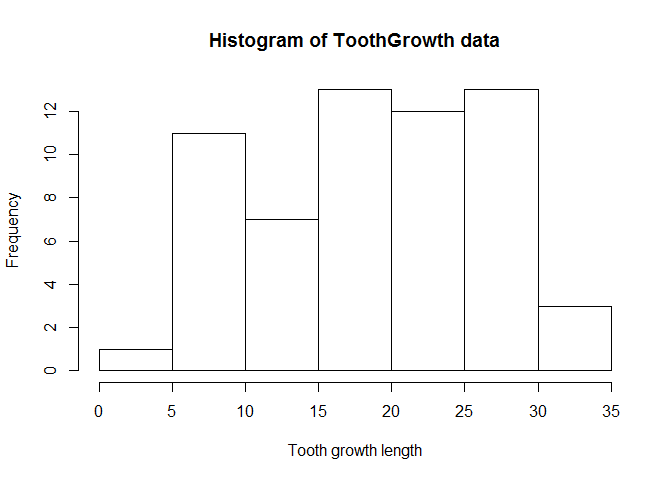
\includegraphics{courseproject_part2_files/figure-latex/unnamed-chunk-1-1.pdf}

\begin{Shaded}
\begin{Highlighting}[]
\CommentTok{# Boxplot of tooth length grouped by delivery methods}
\KeywordTok{ggplot}\NormalTok{(}\KeywordTok{aes}\NormalTok{(}\DataTypeTok{y=}\NormalTok{data}\OperatorTok{$}\NormalTok{len, }\DataTypeTok{x =}\NormalTok{ data}\OperatorTok{$}\NormalTok{supp, }\DataTypeTok{fill =}\NormalTok{ data}\OperatorTok{$}\NormalTok{supp), }\DataTypeTok{data =}\NormalTok{ ToothGrowth) }\OperatorTok{+}\StringTok{ }\KeywordTok{geom_boxplot}\NormalTok{()}\OperatorTok{+}\KeywordTok{labs}\NormalTok{(}\DataTypeTok{title=}\StringTok{"Plot of length by delivery methods"}\NormalTok{, }\DataTypeTok{x =}\StringTok{"Delivery methods"}\NormalTok{, }\DataTypeTok{y =} \StringTok{"Teeth length"}\NormalTok{)}\OperatorTok{+}\StringTok{ }\KeywordTok{scale_fill_discrete}\NormalTok{(}\DataTypeTok{name =} \StringTok{"Delivery Method"}\NormalTok{)}
\end{Highlighting}
\end{Shaded}

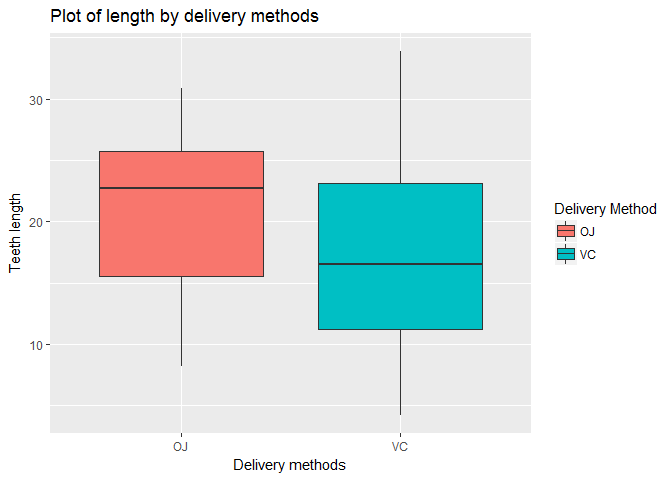
\includegraphics{courseproject_part2_files/figure-latex/unnamed-chunk-1-2.pdf}

\begin{Shaded}
\begin{Highlighting}[]
\CommentTok{# Boxplot of tooth length grouped by dose levels}
\KeywordTok{ggplot}\NormalTok{(}\KeywordTok{aes}\NormalTok{(}\DataTypeTok{y=}\NormalTok{data}\OperatorTok{$}\NormalTok{len, }\DataTypeTok{x =} \KeywordTok{factor}\NormalTok{(data}\OperatorTok{$}\NormalTok{dose), }\DataTypeTok{fill =} \KeywordTok{factor}\NormalTok{(data}\OperatorTok{$}\NormalTok{dose)), }\DataTypeTok{data =}\NormalTok{ ToothGrowth) }\OperatorTok{+}\StringTok{ }\KeywordTok{geom_boxplot}\NormalTok{()}\OperatorTok{+}\KeywordTok{labs}\NormalTok{(}\DataTypeTok{title=}\StringTok{"Plot of length by delivery methods"}\NormalTok{, }\DataTypeTok{x =}\StringTok{"Dose level"}\NormalTok{, }\DataTypeTok{y =} \StringTok{"Teeth length"}\NormalTok{)}\OperatorTok{+}\KeywordTok{scale_fill_discrete}\NormalTok{(}\DataTypeTok{name =} \StringTok{"Dose Level"}\NormalTok{)}
\end{Highlighting}
\end{Shaded}

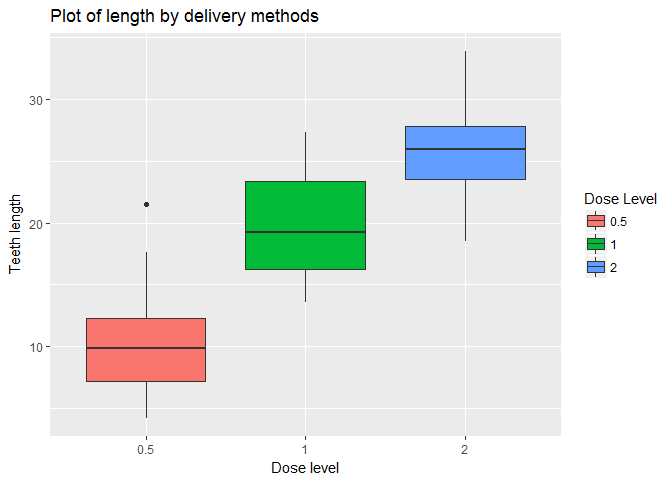
\includegraphics{courseproject_part2_files/figure-latex/unnamed-chunk-1-3.pdf}

For the histogram of the entire toothlength data, we can not observe the
normality of the dataset. However we can see how the delivery methods
and dose level affect the teeth length. The first boxplot hints that
Orange juice delivery method tends to result longer teeth length growth.
The second boxplot indicates that the dose level has positive
relationship with teeth growth.

\subsection{2.2. Effect of the delivery method on tooth growth
data}\label{effect-of-the-delivery-method-on-tooth-growth-data}

In this section, we will use two sample t-test to investigate whether
different delivery methods result statistically significant difference
on the tooth growth length.\\
The null hypothesis will be that there is no significant difference in
the tooth growth between two groups. For this testing, we are using 95\%
of confidence level and equal variance between two groups.

\begin{Shaded}
\begin{Highlighting}[]
\CommentTok{# Sort Toothgrowth data by delivery method}
\NormalTok{VC <-}\StringTok{ }\KeywordTok{subset}\NormalTok{(ToothGrowth, supp}\OperatorTok{==}\StringTok{'VC'}\NormalTok{)}\OperatorTok{$}\NormalTok{len}
\NormalTok{OJ <-}\StringTok{ }\KeywordTok{subset}\NormalTok{(ToothGrowth, supp}\OperatorTok{==}\StringTok{'OJ'}\NormalTok{)}\OperatorTok{$}\NormalTok{len}
\KeywordTok{t.test}\NormalTok{(VC, OJ, }\DataTypeTok{alternative =} \StringTok{"two.sided"}\NormalTok{, }\DataTypeTok{var.equal =} \OtherTok{FALSE}\NormalTok{)}
\end{Highlighting}
\end{Shaded}

\begin{verbatim}
## 
##  Welch Two Sample t-test
## 
## data:  VC and OJ
## t = -1.9153, df = 55.309, p-value = 0.06063
## alternative hypothesis: true difference in means is not equal to 0
## 95 percent confidence interval:
##  -7.5710156  0.1710156
## sample estimates:
## mean of x mean of y 
##  16.96333  20.66333
\end{verbatim}

From the two sample t-test, we can see that the p-value is bigger than
the level of significance (0.06063 \textgreater{} 0.05). Therefore we
fail to reject null hypothesis, and this indicates that there is no
significant difference between the delivery method groups, VC and OJ.

\subsection{2.3. Effect of the dose level on tooth growth
data}\label{effect-of-the-dose-level-on-tooth-growth-data}

In this section, we will use two sample t-test to investigate whether
different dose level result statistically significant difference on the
tooth growth length.\\
The null hypothesis will be that there is no significant difference in
the tooth growth between two groups (dose level 0.5 and dose level 2).
For this testing, we are using 95\% of confidence level and equal
variance between two groups.

\begin{Shaded}
\begin{Highlighting}[]
\CommentTok{# Sort Toothgrowth data by delivery method}
\NormalTok{dose0.}\DecValTok{5}\NormalTok{ <-}\StringTok{ }\KeywordTok{subset}\NormalTok{(ToothGrowth, dose}\OperatorTok{==}\FloatTok{0.5}\NormalTok{)}\OperatorTok{$}\NormalTok{len}
\NormalTok{dose2.}\DecValTok{0}\NormalTok{<-}\StringTok{ }\KeywordTok{subset}\NormalTok{(ToothGrowth, dose}\OperatorTok{==}\DecValTok{2}\NormalTok{)}\OperatorTok{$}\NormalTok{len}
\KeywordTok{t.test}\NormalTok{(dose0.}\DecValTok{5}\NormalTok{, dose2.}\DecValTok{0}\NormalTok{, }\DataTypeTok{alternative =} \StringTok{"two.sided"}\NormalTok{, }\DataTypeTok{var.equal =} \OtherTok{FALSE}\NormalTok{)}
\end{Highlighting}
\end{Shaded}

\begin{verbatim}
## 
##  Welch Two Sample t-test
## 
## data:  dose0.5 and dose2.0
## t = -11.799, df = 36.883, p-value = 4.398e-14
## alternative hypothesis: true difference in means is not equal to 0
## 95 percent confidence interval:
##  -18.15617 -12.83383
## sample estimates:
## mean of x mean of y 
##    10.605    26.100
\end{verbatim}

From the two sample t-test, we can see that the p-value is much smaller
than the level of significance (4.398e-14 \textless{} 0.05). Therefore
we successfully reject null hypothesis. This indicates that there is
significant difference between the dose level groups.


\end{document}
